\subsection{Utente non autenticato}
\subsubsection{Panoramica utente non autenticato}
DA FARE
\begin{figure}[H]
\centering
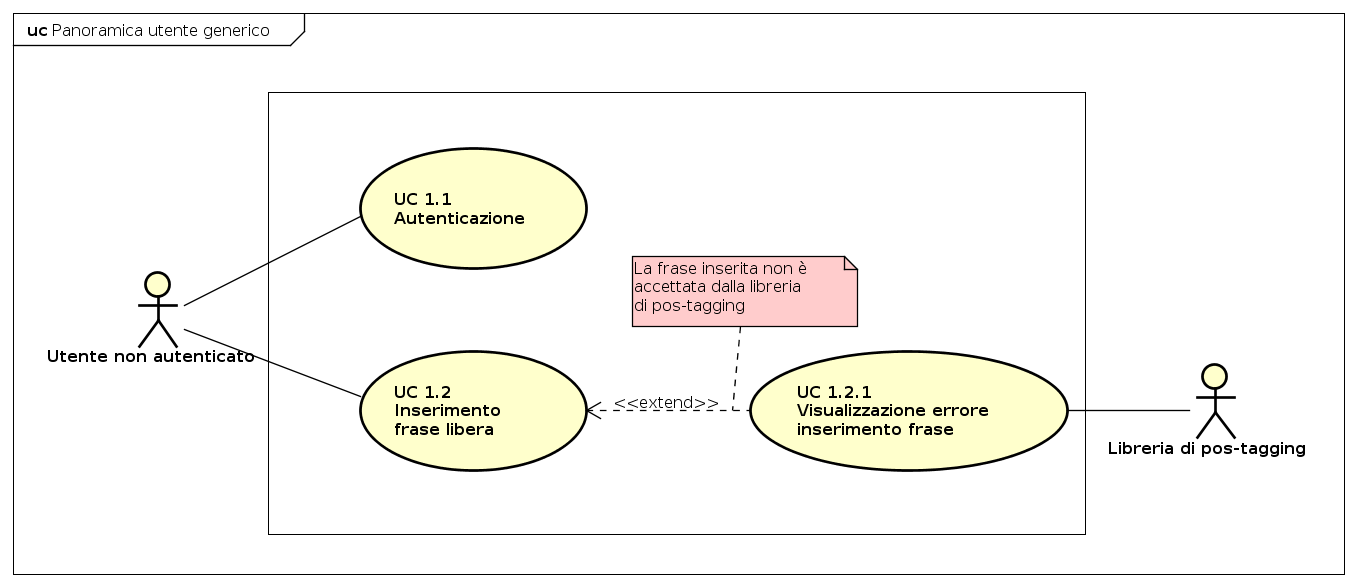
\includegraphics[width=17cm]{img/PanoramicaUtenteGenerico.png} 
\caption{Panoramica utente generico}\label{fig:1}
\end{figure}


\subsubsection{UC 1.1 - Autenticazione}
\begin{figure}[H]
\centering
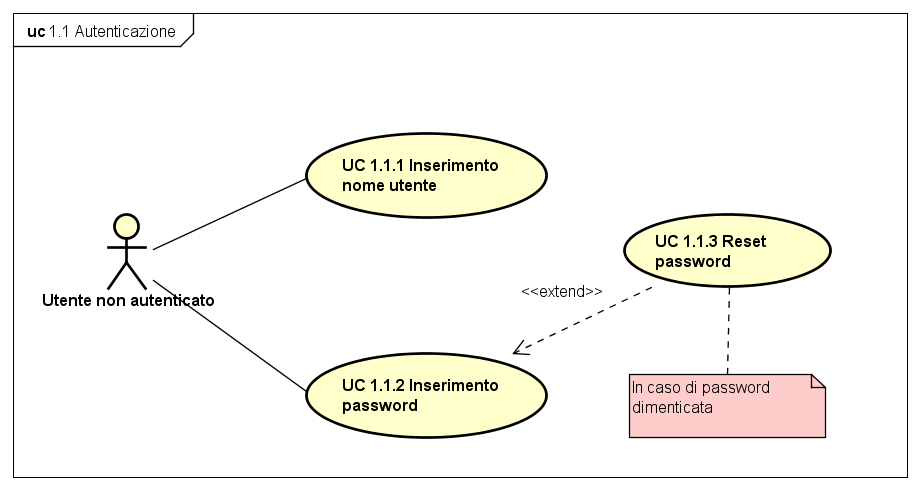
\includegraphics[width=17cm]{img/UC11.png} 
\caption{Caso d'uso 1.1}\label{fig:11}
\end{figure}
\begin{itemize}
\item[•]\textbf{Attori}: Utente non autenticato;
\item[•]\textbf{Descrizione}:  L’utente non identificato inserisce username e password e si autentica accedendo alla dashboard;
\item[•]\textbf{Precondizione}: L’utente non è autenticato;
\item[•]\textbf{Postcondizione}: L’utente viene autenticato all’interno del sistema;
\item[•]\textbf{Flusso degli eventi principale}:
\begin{enumerate}
\item UC 1.1.1 - Inserimento nome utente;
\item UC 1.1.2 - Inserimento password.
\end{enumerate}
\item[•]\textbf{Estensioni}:
\begin{enumerate}
\item Errore inserimento nome utente con relativo messaggio d’errore;
\item Errore inserimento password con relativo messaggio d’errore.
\end{enumerate}
\end{itemize}

\subsubsection{UC 1.1.1 - Inserimento nome utente}
\begin{itemize}
\item[•]\textbf{Attori}: Utente non autenticato;
\item[•]\textbf{Descrizione}: L’utente inserisce un nome utente durante la registrazione;
\item[•]\textbf{Precondizione}: L’utente non è autenticato;
\item[•]\textbf{Postcondizione}: L’utente ha inserito un nome utente;
\end{itemize}

\subsubsection{UC 1.1.2 - Inserimento password}
\begin{itemize}
\item[•]\textbf{Attori}: Utente non autenticato;
\item[•]\textbf{Descrizione}: L’utente inserisce una password durante la registrazione;
\item[•]\textbf{Precondizione}: L'utente non è autenticato;
\item[•]\textbf{Postcondizione}: L'utente ha inserito una password;
\end{itemize}

%\subsubsection{UC 1.2 - Inserimento frase libera}
%\begin{figure}[H]
%\centering
%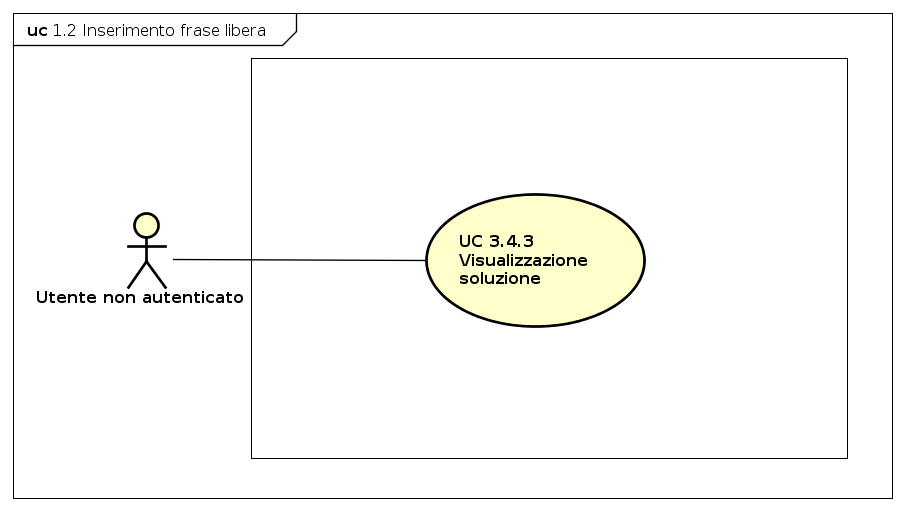
\includegraphics[width=17cm]{img/UC12.png} 
%\caption{Caso d'uso 1.2}\label{fig:12}
%\end{figure}
%\begin{itemize}
%\item[•]\textbf{Attori}: Utente non autenticato;
%\item[•]\textbf{Descrizione}: L'allievo inserisce la propria frase in modo da ricevere l'analisi grammaticale di essa;
%\item[•]\textbf{Precondizione}: Il sistema offre la possibilità di inserire una frase;
%\item[•]\textbf{Postcondizione}: Una frase è stata correttamente inserita;
%\item[•]\textbf{Flusso degli eventi principale}:
%\begin{enumerate}
%\item UC 3.4.3 - Visualizzazione soluzione.
%\end{enumerate}
%\item[•]\textbf{Estensioni}:
%\begin{enumerate}
%\item UC 1.2.1 - Visualizzazione errore inserimento frase.
%\end{enumerate}
%\end{itemize}

%\subsubsection{UC 1.2.1 - Visualizzazione errore inserimento frase}
%\begin{itemize}
%\item[•]\textbf{Attori}: Utente non autenticato, Libreria di pos-tagging;
%\item[•]\textbf{Descrizione}: La frase inserita non è accettata dalla libreria di pos-tagging. L'allievo visualizza un errore e può inserire una nuova frase;
%\item[•]\textbf{Precondizione}: L'allievo ha provato ad inserire una frase;
%\item[•]\textbf{Postcondizione}: L'allievo ha visualizzato il messaggio di errore e può inserire una nuova frase;
%\end{itemize}

\subsubsection{UC 1.2 - Registrazione utente}
\begin{figure}[H]
	\centering
	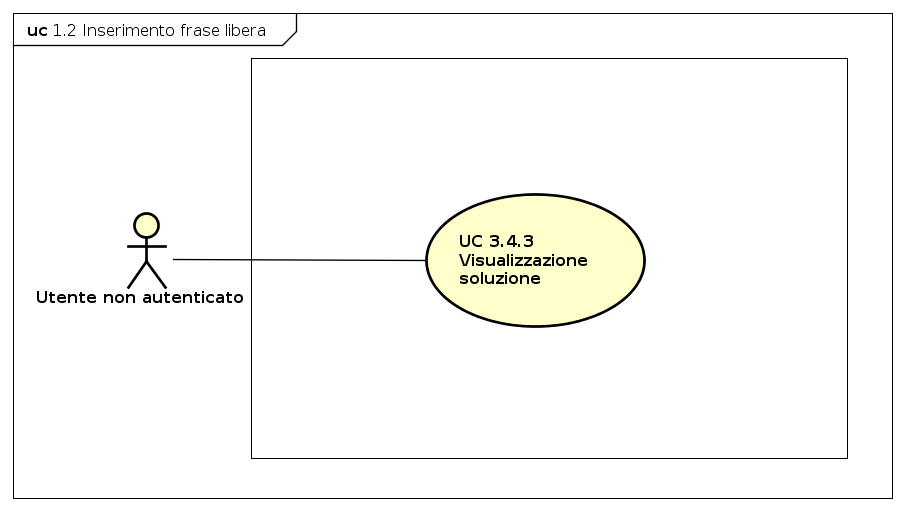
\includegraphics[width=17cm]{img/UC12.png} 
	\caption{Caso d'uso 1.2}\label{fig:12}
\end{figure}
\begin{itemize}
	\item[•]\textbf{Attori}: Utente non registrato;
	\item[•]\textbf{Descrizione}: L'utente non registrato compila il modulo di registrazione al fine di poter accedere al sistema;
	\item[•]\textbf{Precondizione}: L'utente non è registrato;
	\item[•]\textbf{Postcondizione}: L'utente si è registrato e può quindi accedere al sistema;
	\item[•]\textbf{Flusso degli eventi principale}:
	\begin{enumerate}
		\item UC 1.2.3 - Inserimento nome utente;
		\item UC 1.2.4 - Inserimento email;
		\item UC 1.2.5 - Inserimento password;
		\item UC 1.2.6 - Inserimento conferma password;
		\item UC 1.2.7 - Inserimento data di nascita;
		\item UC 1.2.8 - Selezione ruolo;
	\end{enumerate}
	\item[•]\textbf{Estensioni}:
	\begin{enumerate}
		\item UC 1.2.1 - Visualizzazione messaggio errore dato presente;
		\item UC 1.2.2 - Visualizzazione messaggio errore password diverse
	\end{enumerate}
\end{itemize}

\subsubsection{UC 1.2.1 - Visualizzazione messaggio errore dato presente}
\begin{itemize}
	\item[•]\textbf{Attori}: Utente non registrato;
	\item[•]\textbf{Descrizione}: L'utente non registrato visualizza un messaggio di errore relativo all'inserimento
di un dato già presente nel sistema;
	\item[•]\textbf{Precondizione}: L'utente non registrato sta completando la procedura di registrazione;
	\item[•]\textbf{Postcondizione}: L'utente visualizza un messaggio di errore relativo all'inserimento di un valore già presente nel sistema;
	\item[•]\textbf{Flusso degli eventi principale}: L'utente inserisce una email o un nome utente già presente nel sistema, pertanto riceve un messaggio di errore.
\end{itemize}

\subsubsection{UC 1.2.2 - Visualizzazione messaggio errore password diverse}
\begin{itemize}
	\item[•]\textbf{Attori}: Utente non registrato;
	\item[•]\textbf{Descrizione}: L'utente non registrato visualizza un messaggio che comunica che i valori della password e di conferma password sono tra loro diversi;
	\item[•]\textbf{Precondizione}: L'utente non registrato ha inserito la password e la conferma password con valori differenti;
	\item[•]\textbf{Postcondizione}: L'utente visualizza un messaggio di errore relativo all'inserimento di password e conferma password con valori diversi;
	\item[•]\textbf{Flusso degli eventi principale}: L'utente inserisce password e conferma password con valori diversi, pertanto riceve un messaggio di errore.
\end{itemize}

%\subsubsection{UC 1.4 - Richiesta registrazione Sviluppatore}
%\begin{itemize}
%	\item[•]\textbf{Attori}: Utente non autenticato;
%	\item[•]\textbf{Descrizione}: L'utente non identificato, che intende registrarsi come sviluppatore per poter accedere ai dati nella piattaforma, richiede di potersi registrare nel sistema;
%	\item[•]\textbf{Precondizione}: L'utente non è registrato;
%	\item[•]\textbf{Postcondizione}: L'utente ha effettuato la richiesta per registrarsi nell'applicativo;
%	\item[•]\textbf{Flusso degli eventi principale}: L'utente seleziona l'opzione per effettuare la richiesta di registrazione di sviluppatore e la conferma.
%\end{itemize}

\subsubsection{UC 1.2.3 - Inserimento nome utente}
\begin{itemize}
	\item[•]\textbf{Attori}: Utente non registrato;
	\item[•]\textbf{Descrizione}: L'utente inserisce un nome utente durante la registrazione;
	\item[•]\textbf{Precondizione}: L'utente non è registrato;
	\item[•]\textbf{Postcondizione}: L'utente ha inserito un nome utente;
\end{itemize}

\subsubsection{UC 1.2.4 - Inserimento email istituzionale}
\begin{itemize}
	\item[•]\textbf{Attori}: Utente non registrato;
	\item[•]\textbf{Descrizione}: L'utente inserisce la sua email istituzionale durante la registrazione;
	\item[•]\textbf{Precondizione}: L'utente non è registrato;
	\item[•]\textbf{Postcondizione}: L'utente ha inserito una email istituzionale;
\end{itemize}

\subsubsection{UC 1.2.5 - Inserimento password}
\begin{itemize}
	\item[•]\textbf{Attori}: Utente non registrato;
	\item[•]\textbf{Descrizione}: L'utente inserisce una password durante la registrazione;
	\item[•]\textbf{Precondizione}: L'utente non è registrato;
	\item[•]\textbf{Postcondizione}: L'utente ha inserito una password;
\end{itemize}

\subsubsection{UC 1.2.6 - Inserimento conferma password}
\begin{itemize}
	\item[•]\textbf{Attori}: Utente non registrato;
	\item[•]\textbf{Descrizione}: L'utente inserisce la conferma della password durante la registrazione;
	\item[•]\textbf{Precondizione}: L'utente non è registrato;
	\item[•]\textbf{Postcondizione}: L'utente ha inserito la conferma della password;
\end{itemize}

\subsubsection{UC 1.2.7 - Inserimento data di nascita}
\begin{itemize}
	\item[•]\textbf{Attori}: Utente non registrato;
	\item[•]\textbf{Descrizione}: L'utente inserisce la sua data di nascita durante la registrazione;
	\item[•]\textbf{Precondizione}: L'utente non è registrato;
	\item[•]\textbf{Postcondizione}: L'utente ha inserito la sua data di nascita;
\end{itemize}

\subsubsection{UC 1.2.8 - Selezione ruolo}
\begin{itemize}
	\item[•]\textbf{Attori}: Utente non registrato;
	\item[•]\textbf{Descrizione}: L'utente seleziona il ruolo desiderato all'interno del sistema;
	\item[•]\textbf{Precondizione}: L'utente non è registrato e il suo ruolo non è selezionato;
	\item[•]\textbf{Postcondizione}: L'utente ha selezionato il ruolo desiderato;
\end{itemize}
